% IEEE S&P (Oakland), Systematization of Knowledge track.
% Two-column IEEEtran. The classification tables are wide and run over several
% pages, so they sit in a one-column landscape block of their own; longtable
% cannot break across a two-column float.
\documentclass[conference,compsoc]{IEEEtran}
\IEEEoverridecommandlockouts

\usepackage[utf8]{inputenc}
\usepackage[T1]{fontenc}
% tectonic's engine is XeTeX, so inputenc's utf8 option is a no-op and
% \DeclareUnicodeCharacter is undefined. Non-ASCII glyphs are written as LaTeX
% commands at the source (---, \k{a}, \.I) rather than as literal bytes.

\usepackage{amsmath,amssymb,amsthm}
\usepackage{booktabs}
\usepackage{longtable}
\usepackage{pdflscape}
\usepackage{microtype}
\usepackage{graphicx}
\usepackage[hidelinks]{hyperref}

\newtheorem{definition}{Definition}
\newtheorem{theorem}{Theorem}

% One number, one place. Every number in the paper comes from here, and every
% macro here comes from a counted pass over the corpus or over wiki/sources.
% Regenerate the corpus counts with tools/corpus-counts.sh.

% Corpus, counted 2026-08-22.
\newcommand{\NumPapers}{206}          % PDFs in raw/
\newcommand{\NumSources}{200}         % source pages in wiki/sources/
\newcommand{\NumConcepts}{83}
\newcommand{\NumEntities}{116}

% Mapping results. Filled by the Part V generator; do not hand-edit.
\newcommand{\NumUnstated}{37}          % works stating no budget for any party
\newcommand{\NumPriced}{163}         % works bounding at least one party

% --- Numbers used in Part I. Each traces to a wiki source page that was
% --- verified against the primary PDF in the 2026-08-22 audit.
% mia-from-first-principles, blind-baselines-beat-mia, sok-mia-llms-rushing-nowhere,
% do-mias-work-on-llms
\newcommand{\MIAnewMethods}{ten}      % new MIA methods proposed in 2024 alone
\newcommand{\MIAblindSets}{eight}     % published MI evaluation datasets beaten by blind baselines
\newcommand{\MIAwikiLo}{0.988}        % bag-of-words AUC on WikiMIA, low
\newcommand{\MIAwikiHi}{0.994}        % bag-of-words AUC on WikiMIA, high
\newcommand{\MIAmimirAUC}{0.6}        % ceiling on MIMIR outside GitHub
% obfuscated-gradients
\newcommand{\OGpopulation}{nine}      % non-certified ICLR 2018 defences claiming white-box robustness
\newcommand{\OGobfuscated}{seven}     % of those relying on obfuscated gradients
\newcommand{\OGbrokenFull}{six}
\newcommand{\OGbrokenPart}{one}
% adaptive-attacks-defenses
\newcommand{\AAdefences}{thirteen}
% dos-and-donts-ml-security
\newcommand{\DDpapers}{30}            % papers from CCS, S&P, USENIX Security, NDSS
\newcommand{\DDpitfalls}{ten}
\newcommand{\DDminPitfalls}{three}    % pitfalls affecting every one of the 30
% sok-black-box-attack-pitfalls
\newcommand{\BBattacks}{164}
\newcommand{\BBmajorVenue}{102}
\newcommand{\BBrerun}{eleven}          % transfer attacks re-run under one time budget
\newcommand{\BBminutes}{30}            % minutes per batch in that re-run

% Corpus breadth, counted over wiki/sources/ front-matter tags on 2026-08-22.
\newcommand{\NumMIApages}{21}         % source pages mentioning membership inference
\newcommand{\NumMIAfamily}{12}        % works whose attack family is membership

% --- Findings read off the classification tables. Counted by tools/collect-cls.py
% --- over notes/classification.tsv on 2026-08-22. Regenerate before submission.
\newcommand{\NumAttackWorks}{103}     % works carrying an attack family
\newcommand{\NumTheoryWorks}{97}      % works carrying none
\newcommand{\NumPhaseAccessCells}{19} % populated cells of 32 in phase x access
\newcommand{\NumPartyUnitCells}{25}   % populated cells of 75 in party x unit
\newcommand{\AttackAccessNamed}{72}   % attack works naming an access level
\newcommand{\AttackPostHoc}{34}       % of those, attacking a released model
\newcommand{\AttackTestTime}{25}      % of those, at test time
\newcommand{\AttackTrainTime}{12}     % of those, at training time
\newcommand{\AttackQueriesAttacker}{9} % attack works whose adversary is bounded in queries
\newcommand{\AttackSamplesAttacker}{2} % attack works whose adversary is bounded in samples
\newcommand{\NumExponent}{20}         % works stating an exponent in one party's own resource
\newcommand{\AttackUnbound}{27}       % attack works bounding no party
\newcommand{\TheoryUnbound}{10}        % non-attack works bounding no party
\newcommand{\AttackBudget}{36}        % attack works whose bound is a budget
\newcommand{\AttackUnstated}{28}      % attack works stating no tightness
\newcommand{\AttackPoly}{17}
\newcommand{\AttackMeasured}{12}
\newcommand{\AttackClass}{4}
\newcommand{\AttackPerturb}{20}       % attack works bounded by a perturbation radius
\newcommand{\AttackCorrupt}{5}        % attack works bounded by a corruption fraction

% --- Sparse-parity experiment, exp/survey/experiments/, run 2026-08-22.
% Config: k=3, 2-layer ReLU width 100, batch 128, lr 0.01, fresh batches,
% threshold 0.90 test accuracy, 8 seeds per dimension, d in {20,30,40,50,60}.
% Source: canonical_b128.json (regenerate: sparse_parity.py, seeds fixed).
\newcommand{\ParityK}{3}
\newcommand{\ParitySlope}{2.02}       % fitted log-log exponent of median steps vs d
\newcommand{\ParitySeeds}{8}
\newcommand{\ParityDims}{20 to 60}
\newcommand{\ParitySolved}{40 of 40}  % runs reaching threshold within budget
\newcommand{\ParityMedLoD}{1025}      % median steps at d=20
\newcommand{\ParityMedHiD}{9337.5}    % median steps at d=60 (mean of 4th and 5th of 8)
% Probe regime: batch 8, otherwise width 512 lr 0.1; steps at d=30 vs cap at d=60.
\newcommand{\ProbeMedThirty}{6940}
\newcommand{\ProbeCap}{300000}
\newcommand{\ParityThresh}{90\%}

% --- The near-miss set: works whose treatment of a resource does not match how
% --- tightly they state it. Counted 2026-08-27.
\newcommand{\AssessedPredictable}{90}   % per cent predictable from tightness alone
\newcommand{\NearMiss}{19}              % works where the two disagree
\newcommand{\NearMissA}{10}             % definitional bound, not treated as the object
\newcommand{\NearMissB}{8}              % measured cost, treated deliberately
\newcommand{\NearMissC}{1}              % quantity present, no tightness at all

% --- Baseline column, countable after the re-pass of 2026-08-27.
\newcommand{\BaselineCrit}{50}
\newcommand{\BaselineStated}{29}
\newcommand{\BaselineAbsent}{21}
\newcommand{\BaselineNA}{133}
\newcommand{\BaselineChanged}{31}
\newcommand{\NumRelative}{18}
\newcommand{\NumRelativeAttack}{6}
\newcommand{\NumFlops}{5}
\newcommand{\AttackTimeAttacker}{17}
\newcommand{\ThmAttack}{71}
\newcommand{\ThmOther}{87}
\newcommand{\ThmAttackUnbound}{12}
\newcommand{\ThmOtherUnbound}{6}

% --- Added by check-numbers.py --write; computed from the classification.
\newcommand{\RateAttack}{26}
\newcommand{\RateOther}{10}
\newcommand{\RatioUnbound}{2.5}
\newcommand{\DiffLo}{5.5}
\newcommand{\DiffHi}{26.3}
\newcommand{\ThmRatio}{2.5}
\newcommand{\ThmDiffLo}{$-0.2$}
\newcommand{\ThmDiffHi}{20.2}
\newcommand{\NumScaling}{10}
\newcommand{\PhaseAccessTopFive}{62}
\newcommand{\PartyUnitTopFive}{78}
\newcommand{\NearMissAdv}{9}
\newcommand{\NearMissTrain}{5}
\newcommand{\NearMissCap}{5}
\newcommand{\AttackerTimeCirc}{34}
\newcommand{\AttackerCapability}{25}
\newcommand{\AttackerPerturbAll}{20}
\newcommand{\AttackerCorruptAll}{5}
\newcommand{\AttackerMemory}{4}
\newcommand{\LearnerBound}{65}
\newcommand{\LearnerTime}{21}
\newcommand{\LearnerSamples}{17}
\newcommand{\LearnerClass}{16}
\newcommand{\LearnerFlops}{5}
\newcommand{\LearnerOther}{6}
\newcommand{\AuditorBound}{10}
\newcommand{\MechanismBound}{7}
\newcommand{\QuoteOnFile}{172}
\newcommand{\QuoteAbsent}{28}
\newcommand{\QuoteHand}{0}

% --- Second quotation pass, tools/check-quotes.py bound through raw/SOURCES.md, run 2026-09-03.
\newcommand{\QuoteBound}{155}          % quotations verified in their own document
\newcommand{\QuoteUnbound}{5}        % not bound to a document by title, or no prose fragment


\begin{document}

\title{How Hard Is the Attack?\\
A Complexity-Theoretic Systematization of Machine Learning Security}

\author{\IEEEauthorblockN{Halil {\.I}brahim Kanpak}
\IEEEauthorblockA{Ko\c{c} University\\
Istanbul, T\"urkiye}}

\maketitle

% A survey cites what it surveys. Numbering is shared with the supplement,
% which lists every work by the number it carries here.
\nocite{*}

\begin{abstract}
% NOTE: rewritten 2026-08-27 to describe the paper as it stands. The earlier
% version promised an experiment with four coordinates and four empty regions,
% which belong to the formalization section that is not yet written. Restore that
% sentence when that section lands, and not before.
Formal results on the security of machine learning are hard to compare, because a
claim about an attack rarely states what the attacker may spend. We read
\NumSources{} formal works and record, for each one, which party's resources enter
its main claim, in what unit, and how tightly. \NumUnstated{} of them bound no
party at all, and among the \NumAttackWorks{} that study a named attack the rate is
roughly twice that found in the works drawn from cryptography and learning theory.
Where the attack literature does bound an adversary it usually bounds what the
adversary may change, since \AttackBudget{} state a numeric allowance such as a
perturbation radius while \NumExponentAttack{} state a bound relative to an honest
party's work, the form that lets two results share a scale. We identify
\NearMiss{} works holding a resource quantity their own framing does not carry, and
report the units in which the two halves of the field price their parties, which
do not overlap.

\end{abstract}

\begin{IEEEkeywords}
machine learning security, threat models, adversary models, computational
hardness, fine-grained cryptography, systematization of knowledge
\end{IEEEkeywords}

\section{Introduction}
\label{sec:intro}

Security claims about machine learning appear faster than the field can compare
them. Arp et al.\ read \DDpapers{} papers from CCS, S\&P, USENIX Security and NDSS
across a decade, name \DDpitfalls{} recurring pitfalls, and find every one of the
\DDpapers{} papers affected by at least \DDminPitfalls{} of them \cite{AQPWPWCR22}.
One of the \DDpitfalls{} is the threat model. Their measurement is of practice, and
the same defect shows up in the results themselves wherever one attack has been
studied by several groups.

Membership inference makes the defect concrete, and we use it to state the three
problems in Section~\ref{sec:problem}. The attack decides whether one record was in
a model's training set, and Meeus et al.\ count at least \MIAnewMethods{} new
methods for it proposed in 2024 alone \cite{MSJFRM25}. The published verdicts on whether it works span the full range.
Carlini et al.\ report that it succeeds at low false positive rates
\cite{CCNSTT22}. Duan et al.\ run five attacks against models whose training set is
known and report that none exceeds \MIAmimirAUC{} AUC outside one domain
\cite{DSMMSZTCEH24}. Das et al.\ report that on \MIAblindSets{} published
benchmarks a classifier that never queries the model beats the best attack that
does \cite{DZT25}. Zhang et al.\ argue that the attack cannot establish training-set
membership for a deployed model at all \cite{ZDKT25}. Every one of these results is
correct on its own terms. They differ in what they let the attacker know and spend,
and none of them states that in a form the others can be checked against.

Membership inference is one attack among many, and it appears in \NumMIApages{} of
the \NumSources{} works surveyed here. The corpus also covers evasion, poisoning,
backdoors, data reconstruction and model extraction, and on the other side
computational differential privacy, statistical-query and low-degree hardness,
bounded-memory adversaries and fine-grained cryptography. No single attack runs
through every part of the survey, so each part of Section~\ref{sec:landscape}
carries its own worked case.

The field has not ignored the adversary. It has described the adversary without
pricing it. The standing systematization of the area sorts attacks by the stage of
the pipeline the adversary acts at, whether it can write as well as read, the
access it holds, and the goal it pursues \cite{PMSW18}, and none of those four axes
is a computational resource. Three later systematizations, all of them preprints at the time
of writing, report that their own subfield lacks a formal definition of attack
success, on adversarial examples \cite{FK24}, on model extraction \cite{SSEP24},
and on data reconstruction \cite{WLBZ25}. Each proposes a repair, and each repair supplies knowledge, access
or a success metric. None supplies a budget. A reader holding two results therefore
cannot ask which adversary was stronger, because neither result answers it.

Cryptography has priced adversaries for fifty years, and the objects the comparison
needs already exist there. An adversary class fixes what the attacker may run. A
budget fixes how much of it the attacker may spend. A success criterion with a
tolerance fixes what counts as winning. A baseline fixes what public knowledge
alone already achieves, so that an advantage is measured against something. We
carry those four objects into machine learning security and use them to read the
field.

We read \NumSources{} formal works and record, for each one, which party's
resources enter its main claim and in what unit. Recording the budget per party
rather than per adversary is what lets a single statement hold a bound on the
attacker, a bound on the learner, a bound on an auditor, and a ratio between two of
them. It also makes the most common answer visible, which is that no party's
resources enter the claim at all.

Our contributions are the following.

\begin{itemize}
  \item A survey of \NumSources{} formal works on the security and privacy of
        learning, organized by the attack family together with the party each work
        constrains, recording for every work which party's resources enter its main
        claim, in what unit, and whether the work assesses the adversary explicitly
        or leaves the assessment implicit (Section~\ref{sec:landscape}).
  \item An experiment, $\mathrm{Exp}[\Pi, L, A, R, \kappa]$, whose four coordinates
        are the adversary's observation point on the chain from training data to
        model output, the criterion $R$ it must satisfy and the tolerance $\eta$ it
        is held to, a capability vector $\kappa$ carried per party, and the
        baseline. We show which published results each coordinate separates, and
        which results the experiment does not hold
        (Section~\ref{sec:formalization}).
  \item A mapping of the corpus into that experiment, generated from the recorded
        claim quantifier, antecedent and adversary bound of each work rather than
        assembled by hand, so that it can be rebuilt when the corpus changes
        (Section~\ref{sec:mapping}).
  \item Four regions of the experiment that no work in the corpus occupies, each
        reported with the search that established it rather than as an assertion,
        together with the count of works that state no budget for any party
        (Section~\ref{sec:findings}).
\end{itemize}

\section{Three problems}
\label{sec:problem}

We state three problems. Problem 1 is that one literature reaches incompatible
conclusions about a single attack. Problem 2 is that two literatures define the
same quantity and neither cites the other. Problem 3 is that a stated threat model
does not constrain the attack it was written for. Section~\ref{sec:problem-cause}
takes the three in turn and shows that one absence produces all of them.

\subsection{Problem 1: incompatible conclusions within one literature}
\label{sec:problem-one}

Membership inference decides whether one record was in a model's training set.
Meeus et al.\ count at least \MIAnewMethods{} new methods for it proposed in 2024
alone \cite{MSJFRM25}, and the four verdicts quoted in Section~\ref{sec:intro} span
the whole range from success to unfalsifiability. What produced that spread is
visible once each paper's adversary is written down.

Carlini et al.\ give their adversary data drawn from the target's distribution and
the budget to train many shadow models on it, then compare the target's per-example
loss against the two resulting distributions \cite{CCNSTT22}. Duan et al.\ give
theirs a benchmark whose members and non-members come from the Pile's own train and
test split, which removes the shortcut that a benchmark assembled after training
leaves open \cite{DSMMSZTCEH24}. Das et al.\ give theirs no model access at all,
and it still wins, which places the signal in the benchmark rather than in the
model \cite{DZT25}. Meeus et al.\ locate that signal precisely, reporting
\MIAwikiLo{} to \MIAwikiHi{} AUC on WikiMIA from a bag-of-words classifier whose
most predictive features are years \cite{MSJFRM25}.

Zhang et al.\ reach the strongest verdict \cite{ZDKT25}. To bound a false positive
rate, the party running the attack must know the distribution of its test statistic
under the hypothesis that the model was trained without the record in question.
That hypothesis cannot be sampled.

None of the five states a budget in a form the others could be checked
against. The last of them comes closest to stating one. Zhang et al., in a position paper
not yet refereed, give two independent
reasons the null hypothesis cannot be sampled, and the second survives the removal
of the first. Granted full knowledge of the training set and of the training
algorithm, sampling the null ``would still be prohibitively expensive as it would
require training new large models'' \cite{ZDKT25}. That is a security claim
declared unfalsifiable against a party that cannot afford a training run. The paper
names the cost and moves on. It does not record the bound as a parameter, so the
claim cannot be compared with a claim made against a party of any other budget.

\subsection{Problem 2: the attacker-to-honest cost ratio, defined twice without contact}
\label{sec:problem-two}

A proof-of-learning asks a party claiming to have trained a model to produce a
record of the training run, which a verifier then checks \cite{JYCDTCP21}. The
scheme is secure when forging the record costs at least as much as training
honestly. Jia et al.\ state that requirement three times, in the form
$\mathbb{E}[C_A] \geq \mathbb{E}[C_T]$, where $C_A$ is the cost of any spoofing
strategy and $C_T$ the cost of the honest training run.

The inequality carries no exponent, no adversary class, no security parameter and
no assumption. As written it holds by definition for the spoof that simply retrains the
model, and the authors say plainly that they cannot prove it for anything else.
Having concluded in \S VII-B3a that a passing forgery ``would be at least as
computationally expensive as what it took'' the honest trainer, they add two pages
later that ``given that we are not aware of a mechanism to prove this formally, we
present the following as a conjecture'' \cite{JYCDTCP21}.

Fine-grained cryptography defines the same quantity and gives it a name. Brzuska
and Couteau's Definition 6 fixes an $(\varepsilon,\delta)$-fine-grained one-way
function as one that no circuit of size below $|f|^{1+\delta}$ inverts with
non-negligible probability \cite{BC22}. LaVigne, Lincoln and Vassilevska Williams
name the exponent itself, in their Definition 5, as ``the (relative) gap of an
$T(n)$ fine-grained one-way function $f$'' \cite{LLW19}. Around that one constant
they build fine-grained key exchange and fine-grained public-key encryption.

The two literatures are describing the same object. Neither cites the other. The
proof-of-learning line has the quantity in hand and no name for it, so it cannot
say how much more expensive forgery is, and the fine-grained line has the name and
no application to learning, so nothing in it has ever been instantiated on a
training run.

\subsection{Problem 3: threat models stated without a resource bound}
\label{sec:problem-three}

Athalye et al.\ take the \OGpopulation{} non-certified defences accepted at ICLR
2018 that claim white-box robustness \cite{ACW18}. \OGobfuscated{} of them rely on
a phenomenon the authors name obfuscated gradients. \OGbrokenFull{} are
circumvented completely and \OGbrokenPart{} partially, each under the threat model
its own paper stated.

Two years later Tram\`er et al.\ repeat the exercise on \AAdefences{} defences from
ICLR, ICML and NeurIPS, all of which had performed adaptive evaluations
\cite{TCBM20}. They circumvent all \AAdefences{}. Their diagnosis is that they needed nothing
new. In their words, ``the technical tools to evaluate defenses properly
already exist'', and the issue ``is methodological rather than technical''
\cite{TCBM20}.

A defence and its break can both be correct. The threat models in question fix the
perturbation set and the access level, and they say nothing about what the attacker
may compute or about what counts as success. A model that fixes neither of those
does not constrain the attack, so a defence can satisfy it and an attack can
violate the defence without either party making an error.

\subsection{The common cause}
\label{sec:problem-cause}

The three problems share one cause. Most of these works state no budget for any
party, so there is nothing to hold a view about. Researchers holding different
views about what an adversary is would already be an improvement, because such
positions can be compared. Section~\ref{sec:findings} reports how many.

Take the three in turn. In Problem 1 the five membership inference results grant
their adversaries different things, and each verdict follows its grant. Carlini et
al.\ grant the target's distribution and the compute to train shadow models on it.
Duan et al.\ grant a benchmark that removes the shortcut. Das et al.\ grant no
model access at all. The results cannot be ordered, because no two of them price
the same party in the same unit.

In Problem 2 the proof-of-learning line holds the quantity and has no name for it,
while the fine-grained line holds the name and has never instantiated it on a
training run. Neither can find the other by searching, because neither shares
vocabulary with the other. The shared object is a ratio between two parties' work,
and only one of the two literatures writes it as an exponent.

In Problem 3 the threat models fix the perturbation set and the level of access,
and they leave open what the attacker may compute and what counts as success. A
defence can satisfy such a model and an attack can then break the defence, with
neither party in error, because the model never ruled the attack out.

The field has a name for the third case and not for the first two. Arp et al.'s
tenth pitfall, quoted in Section~\ref{sec:intro}, is the threat model, defined as
the case where ``the security of machine learning is not considered, exposing the
system to a variety of attacks, such as poisoning and evasion attacks''
\cite{AQPWPWCR22}. Neither that pitfall nor its recommendations quantify the
adversary by computation, memory, samples or queries. The defect the field
diagnoses in its own threat models is that they are unstated or imprecise, and
never that they are unpriced.

\section{Complexity-theoretic preliminaries}
\label{sec:prelim}

This section introduces the machinery Section~\ref{sec:findings-tables} uses and stops there.
A reader fluent in game-based security definitions and restricted algorithm classes
can move on.

\subsection{Games, advantage, and the baseline}

A security definition in cryptography is a game between a challenger and an
adversary. The challenger samples a secret, the adversary interacts under stated
rules, and the adversary wins when it produces something the definition names. The
adversary's \emph{advantage} is its winning probability minus the probability it
wins without the object under attack.

Membership inference instantiates this. The challenger trains a model on a dataset
that either contains a target record or does not, the adversary sees the model, and
it guesses which. Since the challenger flips a fair coin, an adversary that ignores
the model wins half the time, and half is the baseline that advantage is measured
against.

The baseline belongs to the definition rather than to the evaluation that follows
it. Yeom et al.\ show what happens when it is chosen without care. Under their
membership advantage the two worlds are equiprobable before the model is consulted,
so the marginal quantity is zero by construction and only model access can produce
advantage \cite{YGFJ18}. Balle, Cherubin and Hayes give the constructive form for
reconstruction, where the baseline is the best attack that ignores the model
entirely and the criterion carries a tolerance $\eta$ rather than demanding exact
recovery \cite{BCH22}. Section~\ref{sec:findings-tables} records, for every work, whether a
baseline of either kind is stated.

\subsection{Adversary classes}

A security claim is a statement about some set of algorithms. Six such sets appear
in this corpus.

\emph{Polynomial time} is the default in cryptography. The adversary is a
probabilistic algorithm whose running time is polynomial in a security parameter,
and a scheme is secure when every such algorithm has negligible advantage.

\emph{Circuit size} is the non-uniform version. The adversary is a family of Boolean
circuits, one per input length, and the resource is the number of gates. Non-uniform
adversaries are at least as strong as uniform ones, so a bound against circuits is
the stronger claim.

\emph{Statistical queries} restrict how an algorithm touches data. An SQ algorithm
never sees a sample. It submits a bounded function and receives that function's
expectation over the distribution, accurate to a stated tolerance. Gradient descent
and principal component analysis both fit the model, which is why SQ lower bounds
carry weight in machine learning \cite{FGRVX17}.

\emph{Low-degree polynomials} restrict an algorithm to thresholding a polynomial of
degree at most $D$ in the observations \cite{Wei25}. Under conditions the low-degree
and statistical-query classes agree \cite{BBHLS21}.

\emph{Bounded memory} restricts space rather than time. Raz shows that learning
parity from a stream requires either quadratic memory in the dimension or
exponentially many samples \cite{Raz16}, and the bounded-storage line in
cryptography builds on the same restriction.

\emph{Function classes} restrict the adversary to a hypothesis class rather than a
resource. Chaudhuri, Imola and Machanavajjhala bound an adversary by the class its
attack algorithm is drawn from, rather than by computational power, using
restricted $f$-divergences \cite{CIM19}.

Two of these classes are often treated as interchangeable with running time, and
they are not. Buhai, Hsieh, Jain and Kothari disprove the quasi-polynomial
low-degree conjecture in the regime it was stated, exhibiting planted distributions
with vanishing low-degree advantage whose noisy distinguishing problem is solved far
faster than the conjecture allows \cite{BHJK25}. Their polynomial-time distinguisher
is for a rectangular generalisation, and in the square symmetric regime the running
time is $n^{O(\log^{1/(k-1)} n)}$. Hsieh et al.\ establish the positive counterpart
\cite{HKKLMT26}. A claim resting on a low-degree bound therefore says something
different from a claim resting on a time bound, and Section~\ref{sec:findings-tables} keeps
the two apart.

\subsection{Worst case, average case, and assumptions}

A worst-case claim says no algorithm succeeds on every instance. An average-case
claim says no algorithm succeeds on instances drawn from a stated distribution.
Cryptography needs the second, because a scheme whose keys are hard to break only
occasionally is not a scheme.

A claim is \emph{unconditional} when it holds outright and \emph{conditional} when
it holds under an assumption such as the hardness of factoring, of learning parity
with noise, or of planted clique. Lower bounds against a restricted class are often
unconditional, since the restriction does the work that an assumption would
otherwise do. Brennan and Bresler map the reductions that carry hardness between
average-case problems in this area \cite{BB20}.

\subsection{Reductions}

A reduction from problem $A$ to problem $B$ transforms an algorithm for $B$ into an
algorithm for $A$. It transfers hardness backwards, so hardness of $A$ implies
hardness of $B$. A reduction fails to carry three things that this corpus
sometimes assumes it does. It does not carry across
adversary classes, so a reduction sound against polynomial-time algorithms says
nothing about statistical-query ones. It does not preserve tightness unless the
transformation's own cost is accounted for. And it inherits every antecedent of the
result it starts from.

\subsection{The gap between two parties}

Fine-grained cryptography asks for security against adversaries that exceed the
honest party's resources by a stated factor rather than superpolynomially. Three conventions for that factor appear in this corpus and they are
not interchangeable.

Brzuska and Couteau work in non-uniform circuit size, and their
$(\varepsilon,\delta)$-fine-grained one-way function admits no inverter of size
below $|f|^{1+\delta}$ \cite{BC22}. LaVigne, Lincoln and Vassilevska Williams work
in uniform word-RAM time and name the object, defining the relative gap as the
constant $\delta$ separating an honest cost of $T(n)^{1-\delta}$ from a threshold of
$T(n)$ \cite{LLW19}. Ball, Rosen, Sabin and Vasudevan also work in word-RAM time but
index their error by the adversary's own discount as well as by the input length, so
a single number does not describe their notion \cite{BRSV17}. Degwekar, Vaikuntanathan
and Vasudevan take a fourth route, restricting both parties to a circuit class rather
than relating their costs by an exponent \cite{DVV16}.

One ceiling on how large such a gap can be is often quoted without its scope. Barak
and Mahmoody show that an adversary making $O((n/\delta)^2)$ \emph{oracle queries}
breaks any $n$-query key exchange in the random oracle model, and they note their
adversary runs efficiently in a relativized world where $\mathrm{P} = \mathrm{NP}$
\cite{BM09}. The bound forbids a super-quadratic query gap in an idealized model. It
constrains neither time gaps nor gaps built on structured assumptions.

\subsection{A terminology collision}

In the privacy-preserving machine learning literature, \emph{fine-grained} almost
always means per-user access control. A keyword search returns that sense and not
the complexity-theoretic one. The two bodies of work share a word and nothing else.

\section{Methodology}
\label{sec:method}

\subsection{Corpus}

The corpus holds \NumPapers{} documents, from which \NumSources{} carry a formal
claim and enter the classification. A work is included when three conditions hold.
It concerns learning or something a learning process produced, meaning a model, its
training data, its parameters, its gradients or its outputs. It makes a formal
claim, meaning a theorem, a definition, or a measurement designed to be comparable
across papers. And somebody's resources bear on that claim, in the sense that
deleting every resource restriction would change what the claim says.

The third condition admits two bodies of work with no machine learning content at
all. Fine-grained cryptography enters because it is the only place where the
comparison between an adversary's work and an honest party's is a defined object.
The bounded-storage literature enters on the same grounds, as the formal home of an
adversary limited in space. Both enter as destinations rather than as subject
matter, and Section~\ref{sec:findings-tables} reports that nothing in the machine
learning half of the corpus has travelled to either.

\subsection{Codebook}

Each work is classified on thirteen fields against a fixed vocabulary, so that two
readers assign the same value. Six fields record the attack scenario and threat
model, and seven record what the work assumes about resources.

The vocabulary was revised four times, each revision driven by a classifier
reporting a work it could not place. The revisions are recorded rather than
smoothed away, because their pattern is itself a result. Two of them added values
for bounds that are not computational, namely a perturbation radius, a corruption
fraction and a privacy budget, without which a work that bounds its adversary
non-computationally would have been recorded as bounding nothing. One separated a
second bounded party from one party bounded under two incomparable resource
notions. Eight of the fourteen gaps reported across the whole pass fell in the
single field recording the attack family, which Section~\ref{sec:findings-tables}
returns to.

\subsection{Procedure}

Each work was read first through its catalogue entry, which records the quantifier
of its main claim and the hypothesis that claim rests on, and then through the
primary document wherever that entry was silent on a field. Four rules decide the
cases where a work admits more than one reading. The claim the abstract leads with
decides the row. The constrained party is whoever the bound binds rather than
whoever the paper is about. When two parties are bounded, the computational bound
decides the row and the other party's unit is recorded beside it. A work that
constrains nobody is recorded as constraining nobody, which is an answer and not a
gap.

Every assignment carries the sentence that produced it. For each work the record
holds a verbatim fragment from the source that determines the constrained party,
the unit and the tightness, together with the definition, theorem or section it
came from. Where a work states no bound, the record holds the claim of absence and
the places that were checked before making it, because an unsupported claim of
absence is worth nothing.

\subsection{Verification}

Every quotation was checked against the primary document by extracting its text
and matching a punctuation-independent fragment. Two passes were run. The first,
over the \NumSources{} works then in the corpus, asked whether a quotation
appeared anywhere in the corpus, and found none absent. That question is weaker
than the failure it was meant to catch. A second pass binds each work to its own
document by title and asks whether the quotation appears in \emph{that} document.
It found four works carrying a neighbour's quotation, an off-by-one rotation
within one batch, which the first pass had passed. All four were re-extracted from
their own sources and verified. Of the works the second pass can bind to a
document, 57 verify and none carries another paper's quotation. A further 85 could
not be bound by title, and 25 record an evidenced claim of absence rather than a
quotation.

Eleven entries failed an automated check and all eleven were false alarms, six from
fragments spanning a line break, two from an error in the checker, one from a claim
of absence written as prose, and two from mathematical notation. A single automated
pass is not sufficient evidence that a quotation is absent, and a pass that asks a
weaker question than the failure mode is worse than none, because it returns a clean
report.

\subsection{Threats to validity}

Three limits bear on the counts reported in
Section~\ref{sec:findings-tables}. Each work was classified once rather than by two
independent readers, so the agreement rate between readers is unmeasured, and the
fixed vocabulary and decision rules are what stand in for that measurement.

One field was re-checked in full before being reported. The column recording
whether a work states what an adversary achieves from public knowledge alone was
applied under two readings during the first pass, one asking for the success rate
available without access to the target and one counting any explicit comparison
quantity. Every row was re-read under the narrower definition and
\BaselineChanged{} changed value. Where two readers checked overlapping rows they
agreed on 24 of 27, which is the only inter-reader agreement figure available here.

The field recording the attack family absorbed eight of the fourteen vocabulary
gaps. That field was built around attacks on a deployed model, and the corpus also
contains attacks on a cryptographic primitive, on a communication channel, on a
training distribution and on an agent's control flow. Its categories are therefore
the least reliable of the thirteen, and the grouping used in
Figure~\ref{fig:sankey} collapses them for that reason.

\section{Four findings from the classification}
\label{sec:findings-tables}

\begin{figure*}[t]
\centering
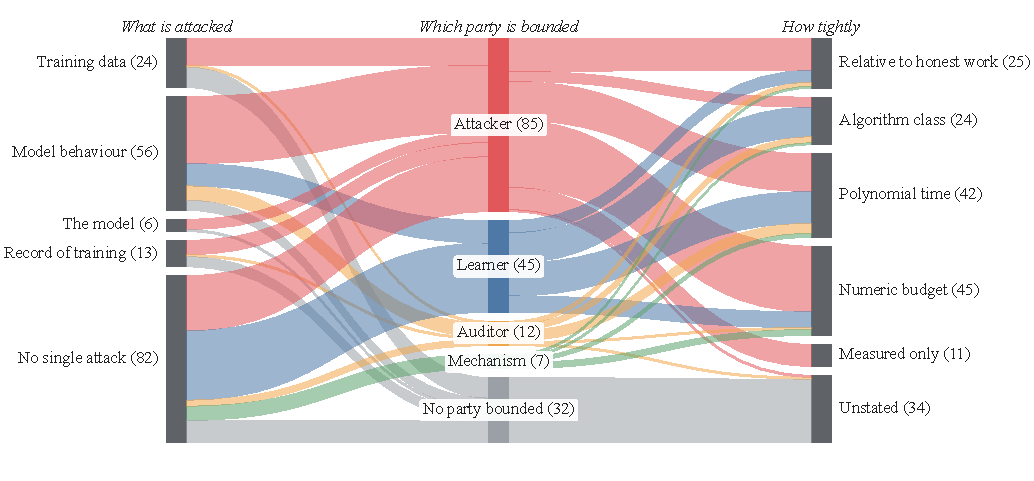
\includegraphics{figures/sankey-corpus}
\caption{The corpus of \NumSources{} works, flowing through what each work
attacks, which party it bounds, and how tightly. Band width is the number of
works and colour is the constrained party. The figure shows three of the thirteen
recorded fields. The full classification is in the supplementary material. Works
with no attack family and works generic over several attacks share the leftmost
band, since neither studies one attack.}
\label{fig:sankey}
\end{figure*}

Figure~\ref{fig:sankey} shows the corpus flowing through three of the recorded
fields. The full classification, on all thirteen fields and with every work named
by citation, is in the supplementary material as six tables. This section reads
them. Each finding names what is dense, what is empty, and what the emptiness
means.

\subsection{The field agrees on access and phase}

The classification by pipeline phase against access level is the one that comes
out full. \NumPhaseAccessCells{} of its 32 cells are populated. Of the \NumAttackWorks{}
works that study an attack, \AttackAccessNamed{} name an access level, and they
split evenly between attacking a model at test time and attacking one already
released. The vocabulary of white box, black box, confidence scores and gradients
is shared, and works from different subfields land in the same cells without
argument.

This is worth establishing before the other three tables, because it shows the
field is capable of agreeing on a threat-model dimension. The disagreement the
rest of this section documents is not a general failure to standardize.

\subsection{It does not agree on resources}

The same corpus against the party each work constrains and the unit it uses fills
\NumPartyUnitCells{} of 75 cells, and the occupied cells do not concentrate. Among the
\NumAttackWorks{} works studying an attack, the adversary is bounded in time in 27
of them, by a perturbation radius in \AttackPerturb{}, in queries in 10, in samples
in 9, and by a corruption fraction in \AttackCorrupt{}. \AttackUnbound{} bound no
party at all.

The row for memory is the one to look at. Four works bound an adversary in memory
and only one of them studies an attack, and that one is bounded-storage
cryptography rather than an attack on a learned model. The bounded-storage
literature has spent two decades on adversaries limited in space, and no work in
this corpus carries that restriction to an adversary attacking a model.

\subsection{The comparable form of bound is almost absent from attack papers}

The third column of Figure~\ref{fig:sankey} sorts the same works by how tightly
each states its bound. \NumExponent{} works state their bound as a relation to an honest party's
work, which is the form that lets two results be placed on one scale.
\NumExponentAttack{} of those \NumExponent{} study an attack, and three of the
\NumExponentAttack{} are cryptographic constructions that happen to carry an attack
family rather than analyses of a deployed system.

The attack literature uses other forms. Of the \NumAttackWorks{} attack works,
\AttackBudget{} state a budget, meaning a numeric allowance such as a perturbation
radius or a query count that carries no relation to anything the defender does.
\AttackUnstated{} state no tightness at all. \AttackPoly{} use the binary
polynomial-time quantifier, \AttackMeasured{} report a measurement with no
definitional standing, and \AttackClass{} name a restricted algorithm class.

A budget bounds what an adversary may change. A relation to honest work bounds what
it must spend to succeed against a defender who spends less. Only the second lets a
reader ask whether one defence costs an attacker more than another, and the corpus
contains \NumExponentAttack{} works that ask it.

\subsection{The attack literature is the half that prices nobody}

Splitting the corpus by whether a work studies a named attack gives the figure's
first column. \AttackUnbound{} of the \NumAttackWorks{} attack works bound no party in
any resource. \TheoryUnbound{} of the \NumTheoryWorks{} works with no attack family
do. Stated as rates, the half of this corpus that studies attacks on machine
learning is about twice as likely to state no adversary bound as the half drawn
from cryptography and learning theory.

The direction is worth stating plainly, because it is the opposite of what a reader
might expect. The cryptographic works in this corpus are not the ones being
imprecise about adversaries. They bound a party in \TheoryUnbound{} fewer cases out
of a smaller total, and when they bound one they more often state the bound in a
form another paper can be compared against.

\subsection{Fifteen works hold a quantity their framing does not carry}

The classification records, separately from how tightly a work states its bound,
whether the work treats that bound as its object or leaves it as a side condition.
Across the corpus the two agree \AssessedPredictable{} per cent of the time, which
is what makes the \NearMiss{} works where they disagree worth naming. Each holds a
resource quantity that its own framing does not carry.

\NearMissA{} of them state a bound in definitional form and do not treat it as the
thing being studied. The filtering impossibility is the clearest. Its theorem turns
on the filter running no faster than the model it audits, which is a ratio between
two parties' compute, and the paper states it as a side condition rather than as the
quantity the result is about \cite{BGGKRR25}. The evaluation guidance that rejects
attacker compute as a threat-model parameter nonetheless fixes a perturbation radius
and reasons about gradient-step counts \cite{CAPBRTGMK19}. Two proof-of-learning
follow-ups price a forgery against honest training and leave the ratio
unparameterized \cite{ZFWCSXZ26}.

\NearMissB{} run the other way, treating a cost deliberately while stating it only
as a measurement. Dziedzic et al.\ calibrate a proof-of-work puzzle to how much a
client has already extracted, which is an adversary priced in compute, with no
definition and no theorem attached \cite{DKLP22}.

The remaining \NearMissC{} state no tightness at all while plainly assessing a
resource. Proof-of-learning requires that forging cost at least as much as training
and states that requirement three times without an exponent, an adversary class or
a security parameter \cite{JYCDTCP21}. The position that membership inference
cannot establish training-set membership rests, in its second and independent
argument, on the cost of sampling a null hypothesis that would require training new
large models \cite{ZDKT25}.

These \NearMiss{} works are where the quantity this survey is about already exists
in the literature without a name.

\subsection{Half the attack literature states no baseline}

An advantage is a success rate minus what public knowledge alone achieves, so a
work that defines adversary success without naming that reference reports a number
with nothing to subtract. \BaselineNA{} of the \NumSources{} works define no
adversary success criterion at all, which is the correct answer for a learning
theory result with no adversary in it. Among the \NumAttackWorks{} works that
study an attack, \BaselineCrit{} define what success means, and of those
\BaselineStated{} name a baseline while \BaselineAbsent{} do not.

This column was the least reliable in the classification and was re-checked in full
before being reported. \BaselineChanged{} of the rows re-checked changed value, and
the errors had four shapes worth naming, because each is a plausible mistake. An
information-theoretic optimum was read as a baseline, when it describes the best any
algorithm could do rather than what an adversary without access achieves. A
previously published accuracy number was read as one, when it describes a different
attack. The cost of an alternative algorithm was read as one. And in an
unforgeability game the raw success tolerance was read as a coin flip, when a search
game has no coin-flip structure at all.

Two independent readers checked overlapping rows and agreed on 24 of 27, which is
the only agreement figure this classification has.

\section{The literature by constrained party}
\label{sec:literature}

Section~\ref{sec:findings-tables} reports how the corpus distributes. This section
says what is in it. The order follows the party each region constrains, because
that is the axis on which the regions differ, and each subsection states what the
region contains, the shape its characteristic result takes, and the boundary that
shape imposes.

\subsection{The attacker bounded in time}

The largest region bounds an adversary in running time or circuit size,
\AttackerTimeCirc{} works in all. Its characteristic result is a guarantee that
holds against every efficient algorithm and against no unbounded one.

Computational differential privacy is the definitional core. Mironov et al.\ relax
the differential privacy guarantee from every distinguisher to every efficient one,
producing the indistinguishability and simulation variants that later work takes as
given \cite{MPRV09}. What that relaxation buys is contested. Groce, Katz and
Yerukhimovich show it buys nothing in the single-curator setting, though their
result is narrower than it is usually quoted as being, applying to black-box
constructions and to queries whose output is a tuple of real numbers of constant
dimension \cite{GKY11}. The authors exclude, by name, queries returning
classifiers, graphs or synthetic databases, which is the case a released model
falls into.

Robustness against a bounded attacker is the region's constructive side. Garg, Jha,
Mahloujifar and Mahmoody wrap a learning problem whose classifier is vulnerable to
every perturbation into one whose classifier resists polynomial-time adversaries
and still yields to unbounded ones, using signatures and error-correcting codes
\cite{GJMM20}. Etesami, Mahloujifar and Mahmoody give a polynomial-time algorithm
that finds, on product distributions under Hamming distance, the close points the
concentration-of-measure bound promises, so there the geometric inevitability of
Section~\ref{sec:lit-none} is attained by an efficient attacker \cite{EMM20}.
Cohen et al.\ define a computational form of reconstruction resilience against
polynomial-time attackers and show that, for training maps that are efficiently
computable and well-spread, it is equivalent to one-wayness \cite{CKMMNST25}.

\subsection{The attacker bounded by what it may change}

The next region, \AttackerCapability{} works, bounds what the adversary may alter
and leaves what it may spend open. \AttackerPerturbAll{} fix a perturbation radius
and \AttackerCorruptAll{} a fraction of the training set.

Certified defences are the mature part. Cohen, Rosenfeld and Kolter certify a radius
around an input within which a smoothed classifier's prediction cannot change
\cite{CRK19}, and Steinhardt, Koh and Liang certify a bound on the loss a poisoning
adversary can induce while controlling a fixed fraction of the data \cite{SKL17}.
Both are guarantees against an adversary with unlimited computation and a limited
reach. The evaluation critiques sit in this region too. Athalye et al.\ and
Tram\`er et al.\ break defences inside their own threat models, and the threat
model each defence stated fixes a radius and nothing else \cite{ACW18,TCBM20}.

That combination is the region's defining feature and its boundary. A radius says
what an attack may do and nothing about what it costs, so two defences certified at
the same radius are indistinguishable under it even when one is far more expensive
to attack. Section~\ref{sec:findings-tables} records that this is the most common
form of adversary bound in the attack literature.

\subsection{The learner bounded}

\LearnerBound{} works constrain the party that trains rather than the party that
attacks. \LearnerTime{} bound it in time, \LearnerSamples{} in samples,
\LearnerClass{} in an algorithm class, \LearnerFlops{} in a budget of
floating-point operations, and \LearnerOther{} in parameters, circuit size, memory
or queries.

The algorithm-class results are the ones that transfer. Feldman et al.\ prove that
statistical-query algorithms need superpolynomially many queries to detect a planted
clique \cite{FGRVX17}, and the low-degree framework gives the same shape of bound
against polynomial thresholds \cite{Wei25,BBHLS21}. Because gradient descent and
principal component analysis are statistical-query algorithms, these bounds apply to
the methods learning actually uses. Bubeck, Price and Razenshteyn use exactly this
to separate robust from ordinary learning, and their separation rests on no
cryptographic assumption at all \cite{BPR19}.

The time-bounded results include the one that runs the implication from robustness
to cryptography. Degwekar, Nakkiran and Vaikuntanathan prove that a task where an
efficient robust classifier exists but cannot be learned efficiently implies
one-way functions \cite{DNV19}. The direction matters and is easy to invert. The
theorem licenses no conclusion from the belief that one-way functions exist, and
what it supports is that a learning task with that hardness profile carries
cryptographic structure rather than arising by accident.

Sample complexity is the second unit. Montasser, Hanneke and Srebro show that every
class of finite VC dimension can be learned under adversarial perturbation, though
not by empirical risk minimization and sometimes at a sample cost exponential in
the VC dimension \cite{MHS19}, and later characterize the sample complexity of the
agnostic case \cite{MHS22}. Nothing in either is computational.

Two results bound the learner in a resource the rest of the corpus does not use.
Bubeck and Sellke show that smoothly interpolating $n$ points in $d$ dimensions
needs about $nd$ parameters, an information-theoretic law with no adversary in it
\cite{BS21}. Raz shows that learning parity from a stream needs either quadratic
memory or exponentially many samples \cite{Raz16}, which is the memory bound the
bounded-storage literature builds on \cite{GZ19}.

\subsection{Nobody bounded}
\label{sec:lit-none}

\NumUnstated{} works constrain no party at all. They are not a residue, and two
distinct lines sit inside them.

The first concludes inevitability from geometry. Mahloujifar, Diochnos and Mahmoody
prove that in a concentrated metric probability space any classifier with constant
error is vulnerable to small perturbations \cite{MDM19}, and Gilmer et al.\ exhibit
the effect on a constructed distribution of two concentric spheres
\cite{GMFSRWG18}. The radius in each theorem is its conclusion, not a restriction
on any adversary. These conclude inevitability precisely because no resource enters
them, which is why the frame of this survey does not hold them and why the survey
says so.

The hypothesis those theorems rest on has been measured. Mahloujifar, Zhang,
Mahmoody and Evans estimate the concentration function on image benchmarks and find
it does not explain observed vulnerability \cite{MZME19}. A conditional theorem
whose antecedent is measured false is a limit on the theorem, not a sibling result,
and the corpus records it as one.

The second line is critique of evaluation and of definition. Das et al.\ show that
classifiers which never query a model beat published membership inference attacks
on eight benchmarks \cite{DZT25}, Arp et al.\ measure the prevalence of ten
pitfalls across four venues \cite{AQPWPWCR22}, and Shafran et al.\ report that
model extraction has no formal definition of success at all \cite{SSEP24}. Balle,
Cherubin and Hayes define reconstruction against an informed adversary and quantify
over every reconstruction attack with no bound on it \cite{BCH22}, which is the
definitional form the critiques ask for, and it prices nobody. These works bound
nobody because their claims are about practice, or about what success means,
rather than about an adversary's cost.

\subsection{The auditor and the mechanism}

\AuditorBound{} works bound an auditor and \MechanismBound{} a mechanism, parties
that neither attack nor learn.

The auditor results are impossibilities about detection. Goldwasser, Kim,
Vaikuntanathan and Zamir plant a backdoor in a classifier so that no polynomial-time
distinguisher with oracle access can tell the backdoored model from an honestly
trained one \cite{GKVZ22}, and the bound sits on the distinguisher, so the
constrained party is whoever audits. Kalavasis et al.\ extend the guarantee to
white-box access under obfuscation, and note that the earlier work leaves that case
open \cite{KKOSVZ24}. Ball et al.\ show there exist language models for which no
efficient prompt filter works, under a construction in which the model shares a
secret key with the attacker \cite{BGGKRR26}. The claim is existential and about
constructed models.

The mechanism results price the defence itself. Bun, Chen and Vadhan separate
computational from statistical differential privacy by exhibiting a polynomial-time
mechanism, so the bound sits on the mechanism \cite{BCV16}. Dinur et al.\ bound the
space a differentially private mechanism may use while remaining sound under
adaptive queries \cite{DSWZ23}, and Ratliff and Vadhan treat the mechanism's own
running time as a leakage channel \cite{RV24}. All three put the resource bound on
the system rather than on anyone attacking it.

\subsection{Where the two halves meet, and do not}

Fine-grained cryptography is where the relation between two parties' work has a
name and a parameter \cite{BC22,LLW19,BRSV17}, and Degwekar, Vaikuntanathan and
Vasudevan restrict both parties to a circuit class instead \cite{DVV16}. It contains
no machine learning. The proof-of-learning line states the same relation with the
exponent fixed at one, as a requirement its authors could not prove
\cite{JYCDTCP21}, a gap their follow-up confirms \cite{FJTYCDCP23}. The
\NumRelativeAttack{} attack works of Table~\ref{tab:relative} each state such a
relation, and none writes it in the fine-grained vocabulary or cites it.

The learning-theory exponents are the closest the machine learning side comes to a
priced adversary. The information exponent \cite{AGJ21}, the leap \cite{ABM23} and
the generative exponent \cite{DPLB24,DLB25} each give a sample threshold defined
against an algorithm class.

Two boundaries on those thresholds are quoted more often than they now hold. The
thresholds were stated for detection rather than recovery, as the single-index
result says of itself \cite{DPLB24}. For polynomial links Lee, Oko, Suzuki and Wu
carry weak recovery through to strong recovery at
$\tilde\Theta(d^{(p^*-1) \vee 1})$ samples, governed by the generative exponent
\cite{LOSW24}, and Glasgow reaches $o(1)$ population error on the Boolean parity
instance in $\tilde\Theta(d)$ \cite{Gla24}. And they were stated for single-pass
training, which batch reuse was reported to escape \cite{DTAPZK24}. Reuse instead
attains the generative exponent in place of the information exponent, because two
steps on one minibatch pass the label through the activation's derivative
\cite{LOSW24,TME25}, and for the plain quadratic activation full-batch reuse gains
nothing at all \cite{KJWSM26}. A security claim resting on either boundary has to
say which version it means.

\subsection{Training compute as a priced resource}

The corpus holds \NumScaling{} works on neural scaling laws, and \NumFlops{} of
them are priced in a budget of floating-point operations spent on training, the
rest in the sample or parameter count that a fixed budget buys. Kaplan et al.\ fit
loss against model size, data and compute \cite{KMHBCCGRWA20}, and Hoffmann et al.\
correct the allocation between model size and data at a fixed budget
\cite{HBMBCRCHWCHNMDDGOSERVS22}. Ho et al.\ measure how much of the observed
improvement comes from better algorithms rather than more compute
\cite{HBEORGATS24}.

None of these works concerns an adversary, and all of them bound the trainer. They
matter to this survey because they establish that the unit exists and is measured.
Shavit's compute-monitoring proposal is the one work in the corpus that carries a
training-compute budget toward a security claim, and it states a hardness
requirement without a construction \cite{Sha23}. Its monitored quantity is
chip-hours rather than operations, which is a further step away from the unit the
scaling literature measures. The gap between a literature that measures training
compute precisely and a security literature that never states an adversary's budget
in it is the widest single gap this corpus contains.

One work crosses in the other direction. Haghifam, Smith and Ullman show a setting
where a membership inference attacker needs many more samples than the training
algorithm used \cite{HSU25}. The separation vanishes when the attacker knows the
covariance, so what it prices is ignorance of the data distribution rather than
attack difficulty as such.

\section{What the mapping shows}
\label{sec:findings}

\subsection{The field's considered rejection}
\label{sec:findings-rejection}

Part of the field has considered pricing the attacker and declined. In a set of
recommendations for evaluating adversarial robustness, circulated as a preprint and
widely adopted without formal publication, Carlini et al.\ write that
there ``are few reasonable threat models under which an attacker can compute 100
iterations of gradient descent, but not 1000'', and conclude that an evaluation
should assume an adversary who spends whatever time is needed \cite{CAPBRTGMK19}.
That is a considered position rather than an oversight, and it is restated from
earlier work by an overlapping set of authors \cite{ACW18}.

The position rejects attacker compute as a restriction imposed inside a fixed
threat model. It does not address attacker compute as the unit in which two claims
are compared, and work in the same area adopts exactly that second use. Suya et
al.\ re-run \BBattacks{} surveyed attacks under a fixed time budget and recommend
that ``execution cost such as the local attack runtime should be used as the
equalizing factor when comparing black-box attack performance, not the number of
iterations'' \cite{SSZHTE24}. Their runtime enters no definition of robustness, so
a defence is still not credited for costing the attacker more.

\section{Related work}
\label{sec:related}

\paragraph{The systematization this survey builds on.}
Papernot, McDaniel, Sinha and Wellman gave the field its standing map of attacks on
machine learning, and most later work in the area still uses its vocabulary
\cite{PMSW18}. Their threat model has three parts: the stage of the pipeline the
adversary attacks, what it is able to do once there, and the goal it pursues. The
middle part takes a different form in each phase, since their Figure 3 places white
box and black box at inference and read and write access at training. We adopt their
attack families wherever they fit, and Section~\ref{sec:tables} adds one axis they
do not carry, which is the resource each work bounds and the party it binds.

\paragraph{Systematizations of one attack family.}
Several later works map a single family in more depth than a general survey allows,
and each reports the same absence from inside its own subfield. Fenaux and
Kerschbaum formalize adversary knowledge for adversarial examples through an oracle
abstraction and a security game, and record a lack of standards for evaluating those
attacks \cite{FK24}. Suya et al.\ place 164 black-box attacks in a four-axis grid and
show that several state-of-the-art claims dissolve once a baseline is given the same
knowledge the new attack assumes \cite{SSZHTE24}. Wen, Liu, Backes and Zhang report
that data reconstruction has no agreed formal definition and supply one with a
tolerance \cite{WLBZ25}. Shafran, Shumailov, Erdogdu and Papernot report the same for
model extraction and disentangle the adversary into prior data, query distribution
and query policy \cite{SSEP24}. Meeus et al.\ do it for membership inference against
language models and show the benchmarks carry a distribution shift a model-free
classifier can exploit \cite{MSJFRM25}. Desfontaines and Pej\'o catalogue the
variants of differential privacy along seven dimensions \cite{DP20}. Each of these
repairs supplies knowledge, access, or a success criterion. None supplies a budget,
and Section~\ref{sec:tables} takes the budget as its organizing question.

\paragraph{Critiques of evaluation practice.}
A second line measures how the field evaluates rather than how it defines. Arp et
al.\ name ten pitfalls in learning-based security, measure their prevalence across
\DDpapers{} papers from four venues over a decade, and survey the authors of those
papers for agreement \cite{AQPWPWCR22}. Athalye, Carlini and Wagner identify
obfuscated gradients and circumvent \OGobfuscated{} of the \OGpopulation{}
non-certified defences at one conference \cite{ACW18}. Tram\`er, Carlini, Brendel and
M\k{a}dry repeat the exercise on \AAdefences{} defences that had all performed
adaptive evaluations, and conclude that the difficulty is methodological rather than
technical \cite{TCBM20}. Carlini et al.\ turn the lesson into a checklist and state a
position this survey returns to in Section~\ref{sec:findings}, that attacker
computation should not be a threat-model parameter \cite{CAPBRTGMK19}. These works
diagnose threat models as unstated or imprecise. None of them diagnoses a threat
model as unpriced, which is the reading Section~\ref{sec:tables} adds.

\paragraph{Where the quantity already has a definition.}
Fine-grained cryptography is the formal home of the comparison between an
adversary's work and an honest party's. Brzuska and Couteau define an
$(\varepsilon,\delta)$-fine-grained one-way function and then argue at length that
the implication they want cannot be proved with current techniques \cite{BC22}.
LaVigne, Lincoln and Vassilevska Williams name the gap as an object and build
fine-grained key exchange and public-key encryption around it \cite{LLW19}. Ball,
Rosen, Sabin and Vasudevan supply average-case fine-grained hardness for the
problems those constructions rest on \cite{BRSV17}, and Degwekar, Vaikuntanathan and
Vasudevan build primitives secure against restricted circuit classes \cite{DVV16}.
This literature contains no machine learning, and Section~\ref{sec:tables} reports
that no work in the machine learning half of the corpus states its adversary in
these terms.

\paragraph{Restricted adversary classes as a security tool.}
Restricting the adversary to an algorithm class, rather than to a running time, has a
record in security. Chaudhuri, Imola and Machanavajjhala bound a privacy adversary by
the function class its attack is drawn from \cite{CIM19}. Goldwasser, Kim,
Vaikuntanathan and Zamir plant backdoors undetectable to any polynomial-time
distinguisher with oracle access \cite{GKVZ22}. Degwekar, Nakkiran and Vaikuntanathan
show that a task where robust classifiers exist but cannot be learned efficiently
implies one-way functions \cite{DNV19}. Jagielski et al.\ price a model-extraction
adversary by algorithm class, showing that extraction expressible as statistical
queries needs exponentially many samples in depth for fidelity extraction
\cite{JCBKP20}, and Chandrasekaran et al.\ give extraction a query budget inside its
definition by reducing it to query-synthesis active learning \cite{CCGJY19}. Dziedzic
et al.\ charge an extraction adversary compute directly, calibrating a proof-of-work
puzzle to how much information a client has already extracted \cite{DKLP22}. These
are the works closest to the question this survey asks, and
Section~\ref{sec:tables} places each of them alongside the rest of the corpus so
that their adversary assumptions can be compared with those of works that state
none.

\section{Conclusion}
\label{sec:conclusion}

A security claim about machine learning is comparable with another when both say
what their adversary may spend. Across \NumSources{} formal works, \NumUnstated{}
state no budget for any party, and among the \NumAttackWorks{} that study a named
attack the figure rises to \AttackUnbound{}, roughly twice the rate found in the
works drawn from cryptography and learning theory.

Where the attack literature does bound an adversary, it usually bounds what the
adversary may change rather than what it must spend. \AttackBudget{} of the
\NumAttackWorks{} attack works state a numeric allowance such as a perturbation
radius. \NumExponentAttack{} state their bound as a relation to an honest party's
work, which is the form that lets two results be placed on one scale.

The vocabulary for the missing form already exists in fine-grained cryptography,
and no work in the machine learning half of this corpus uses it. The same holds for
adversaries bounded in memory, where two decades of cryptographic work has produced
no instance of an adversary attacking a learned model under a space bound.


\bibliographystyle{IEEEtran}
\bibliography{refs}

\end{document}
